\documentclass[tikz, border=10pt]{standalone}
\usepackage{iftex}
\ifluatex
  \usepackage{fontspec}
  \usepackage{unicode-math}
  \setmainfont{Fira Sans}
  \setmonofont{Fira Mono}
  \setmathfont{Fira Math}
  \setmathfont{STIX Two Math}[range={"29F5,"2216}]
\else
  \usepackage[T1]{fontenc}
\fi

\usepackage{amsmath}
\usepackage{tikz}
\usetikzlibrary{arrows.meta}
\tikzset{every node/.style={font=\Large}}

% Theme toggle: \darkbgfalse for light background preview.
\newif\ifdarkbg
\darkbgfalse
\ifdarkbg
  \colorlet{axiscol}{white}
  \colorlet{gridcol}{white!30!black}
  \colorlet{ticklabelcol}{white}
  \colorlet{funcol}{yellow!85!white}
  \colorlet{auxcol}{white!50!black}
\else
  \colorlet{axiscol}{black}
  \colorlet{gridcol}{black!25!white}
  \colorlet{ticklabelcol}{black}
  \colorlet{funcol}{blue!70!black}
  \colorlet{auxcol}{black!40!white}
\fi

% x: -3 to 5   (8 units)   xscale=0.85 → ~6.8 cm wide
% y: -1 to 6   (7 units)   yscale=0.80 → ~5.6 cm tall
% Horizontal asymptote: y = 0 (the x-axis).
% y-intercept: (0, 1/4).  f(-3) ≈ 5.02  f(5) ≈ 0.002
\begin{document}
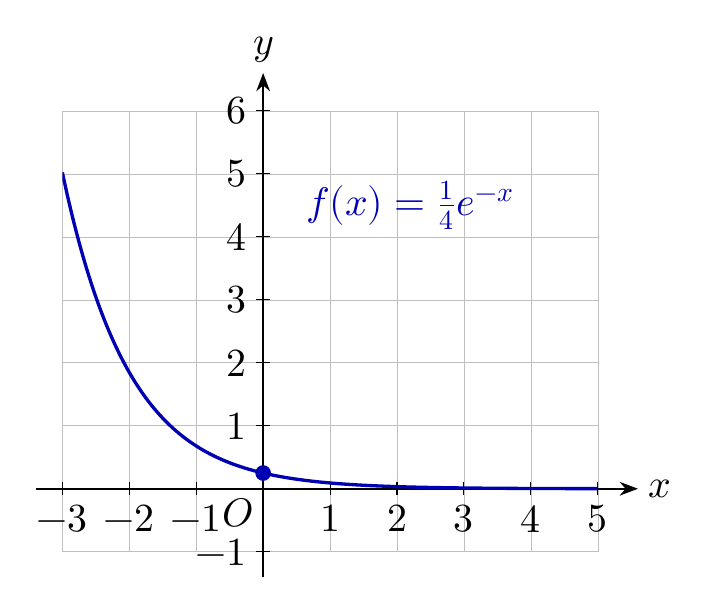
\begin{tikzpicture}[xscale=0.85, yscale=0.80, >=Stealth]

  % Cartesian grid.
  \draw[step=1, very thin, gridcol] (-3,-1) grid (5,6);

  % Axes.
  \draw[->, thick, axiscol] (-3.4,0) -- (5.6,0)
    node[right, text=axiscol] {$x$};
  \draw[->, thick, axiscol] (0,-1.4) -- (0,6.6)
    node[above, text=axiscol] {$y$};

  % Tick marks — x axis.
  \foreach \x in {-3,-2,-1,1,2,3,4,5} {
    \draw[axiscol] (\x, 3pt) -- (\x, -3pt)
      node[below, text=ticklabelcol] {$\x$};
  }

  % Tick marks — y axis (every 1).
  \foreach \y in {-1,1,2,3,4,5,6} {
    \draw[axiscol] (3pt,\y) -- (-3pt,\y)
      node[left, text=ticklabelcol] {$\y$};
  }

  % Origin label.
  \node[below left, text=axiscol] at (0,0) {$O$};

  % Horizontal asymptote label y = 0.
  % \node[below right, text=auxcol, font=\normalsize] at (4.2,0) {$y=0$};

  % Function curve: f(x) = (1/4)·e^(-x), clipped to the window.
  \begin{scope}
    \clip (-3,-1) rectangle (5,6);
    \draw[domain=-3:5, smooth, very thick, funcol, samples=100]
      plot (\x, {0.25*exp(-\x)});
  \end{scope}

  % Function label.
  \node[right, text=funcol] at (0.5,4.5) {$f(x)=\tfrac{1}{4}e^{-x}$};

  % y-intercept (0, 1/4).
  \node[circle, fill=funcol, inner sep=2pt] at (0,0.25) {};
  % \node[above right, text=funcol] at (0,0.25) {$\!\left(0,\,\tfrac{1}{4}\right)$};

\end{tikzpicture}
\end{document}
